\subsection{Niepewność - wyniki eksperymentu z nieznanymi danymi}

Na wykresach \ref{fig:b_ratio_mean}, \ref{fig:d_ratio_mean}, \ref{fig:d_ratio_mean2}, \ref{fig:d_ratio_var2}, \ref{fig:b_ratio_var}, \ref{fig:d_ratio_var} przedstawiono średnie i odchylenia standardowe miary jakości $quality_{ND}$ uzyskane dla poszczególnych konfiguracji eksperymentów. Największa wartość $quality_{ND}$ uzyskana za pomocą Bootstrapa (1.565 dla 5 głów i prawdopodobieństwa 1) jest wyższa niż największa wartość uzyskana za pomocą Dropoutu (1.424 dla 30 wywołań i prawdopodobieństw dropoutu = 0.75). Wyniki bootstrapa dla tych parametrów cechują się trzykrotnie większą wariancją (0.148 a 0.049), ale mimo to sumarycznie wypadają korzystniej od Dropoutu.

Boostrap najlepiej wypada dla małej (5) liczby głów - jest to zaskakujące zachowanie, które może być artefaktem zbyt małej liczby powtórzeń eksperymentu. Podobne wyniki dla różnej liczby głów utrzymują jednak stałą przewagę nad Dropoutem. Zgodna z oczekiwaniami jest przewaga konfiguracji z prawdopodobieństwem uwzględnienia przez głowę próbki równym 1. Dzięki temu poszczególne głowy są lepiej dopasowane do znanych przykładów powiększając różnicę w stosunku do nieznanych danych.

Dla Dropoutu zachodzi podobne zjawisko dla liczby wywołań jak dla głów w Bootstrapie - wbrew oczekiwaniom najlepsze wyniki osiągane są dla mniejszej liczby powtórzeń, przy zachowaniu niewielkich różnic między wartościami. Podobnie zgodnie z oczekiwaniami zachowuje się też drugi z parametrów - prawdopodobieństwo zachowania neuronu w czasie treningu. Wysokie prawdopodobieństwo pozwala ''poznać'' lepiej dane, a prawdopodobieństwo równe 1 uniemożliwia poprawne działanie dropoutu, ponieważ sieć nie jest przyzwyczajona do dropoutu pojawiającego się dopiero w teście.

\begin{figure}[H]
	\begin{floatrow}
		\ffigbox{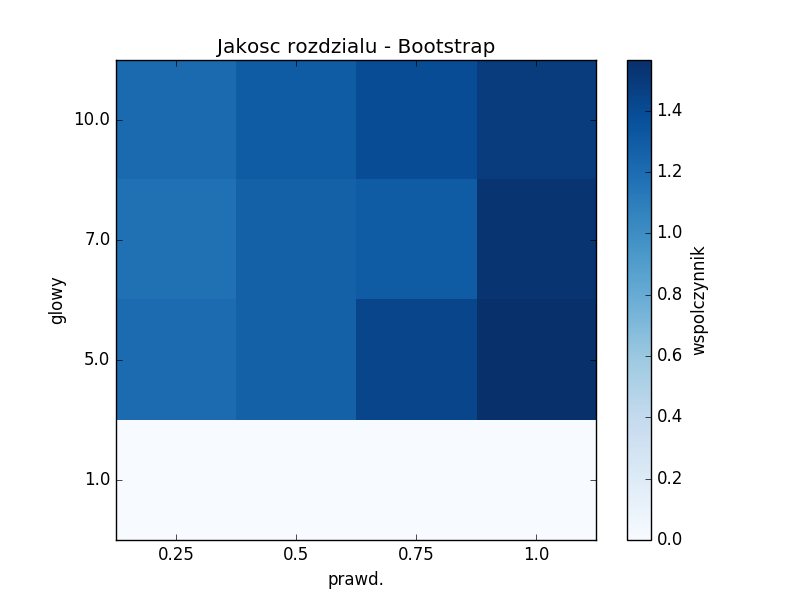
\includegraphics[scale = 0.35]{figures/figures/uncertainties/bootstrap_ratio_mean.png}}{\caption{Bootstrap}\label{fig:b_ratio_mean}}
		\ffigbox{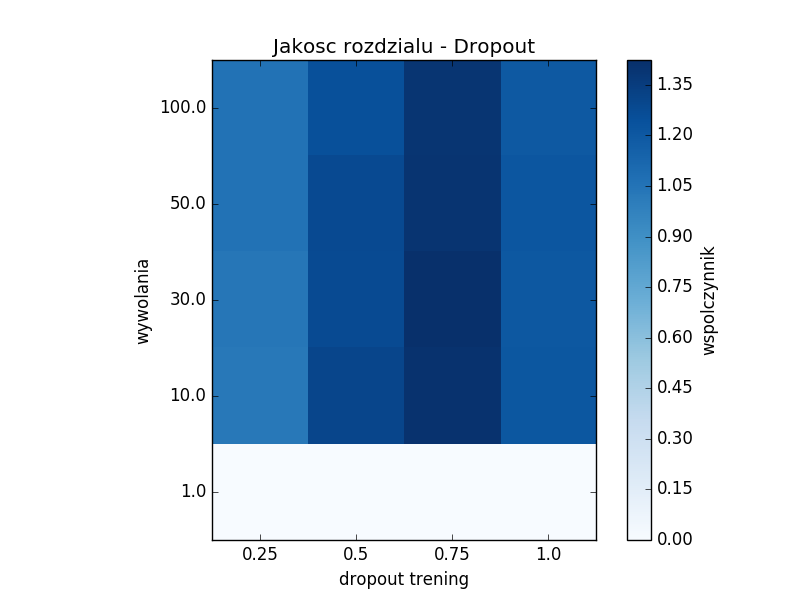
\includegraphics[scale = 0.35]{figures/figures/uncertainties/dropout_ratio_mean.png}}{\caption{Dropout}\label{fig:d_ratio_mean}}
	\end{floatrow}
\end{figure}

\begin{figure}[H]
	\begin{floatrow}
		\ffigbox{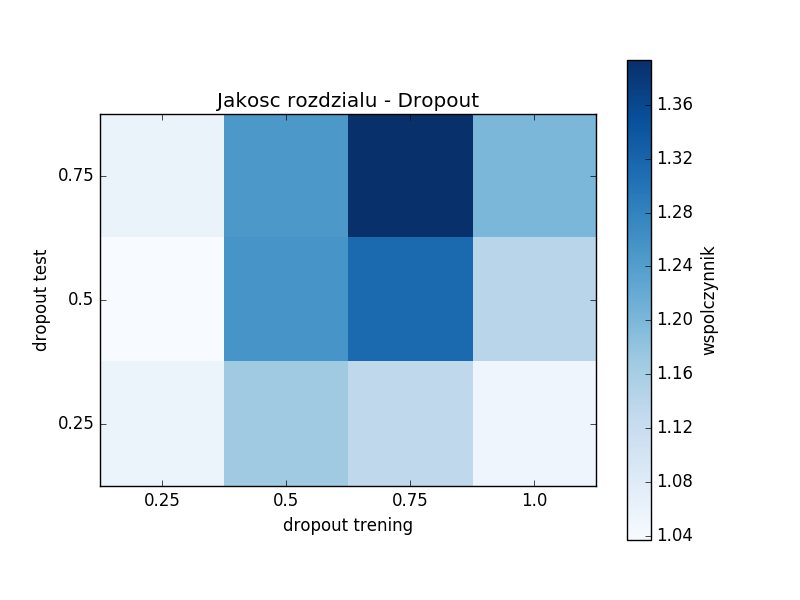
\includegraphics[scale = 0.35]{figures/figures/uncertainties/dropout_ratio_mean2.png}}{\caption{Dropout}\label{fig:d_ratio_mean2}}
		\ffigbox{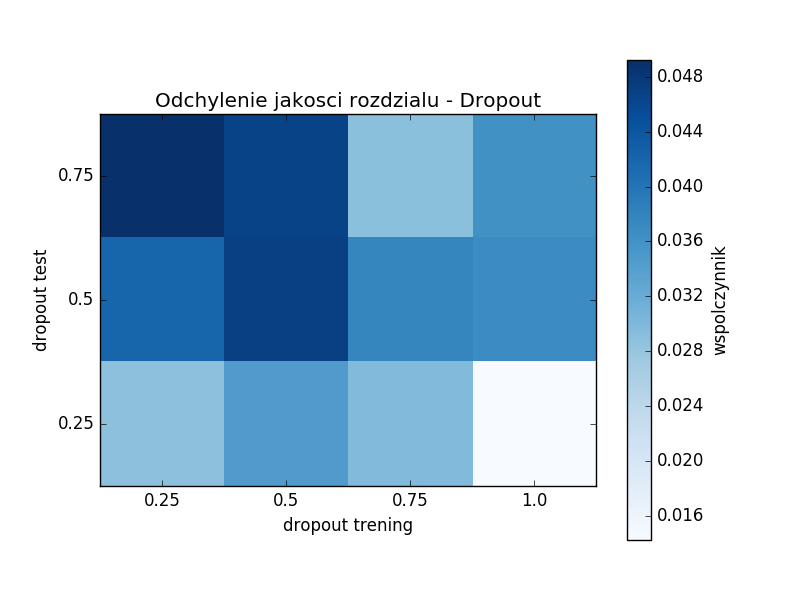
\includegraphics[scale = 0.35]{figures/figures/uncertainties/dropout_ratio_variance2.png}}{\caption{Dropout}\label{fig:d_ratio_var2}}
	\end{floatrow}
\end{figure}

\begin{figure}[H]
	\begin{floatrow}
		\ffigbox{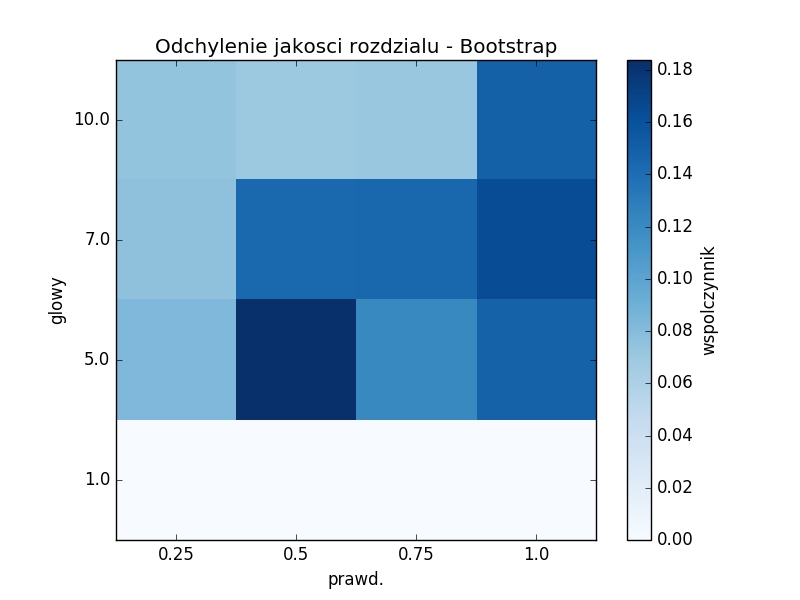
\includegraphics[scale = 0.35]{figures/figures/uncertainties/bootstrap_ratio_variance.png}}{\caption{Bootstrap}\label{fig:b_ratio_var}}
		\ffigbox{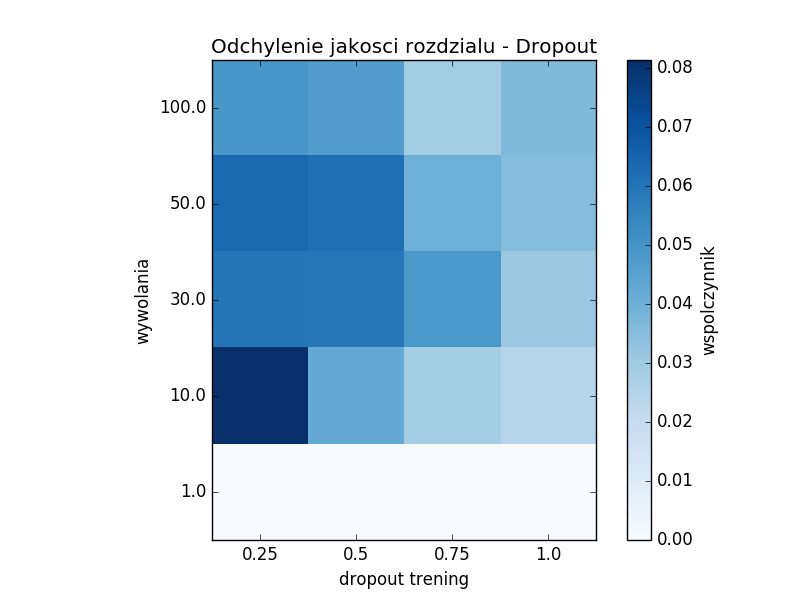
\includegraphics[scale = 0.35]{figures/figures/uncertainties/dropout_ratio_variance.png}}{\caption{Dropout}\label{fig:d_ratio_var}}
	\end{floatrow}
\end{figure}

Na wykresach \ref{fig:b_acc_mean}, \ref{fig:d_acc_mean}, \ref{fig:d_acc_mean2}, \ref{fig:d_acc_var2}, \ref{fig:d_acc_var}, \ref{fig:b_acc_var} przedstawiono średnie i odchylenia standardowe dokładności klasyfikacji uzyskane dla poszczególnych konfiguracji eksperymentów. Wyniki przedstawiają się podobnie jak dla miary $quality_{ND}$. Lepsze wyniki osiąga Bootstrap (44.81\% dla 5 głów i prawdopodobieństwa 0.75, 43.64\%  dla 5 głów i prawdopodobieństwa 1), a jego wyniki są podobne dla wszystkich sensownych parametrów. Wariancja jest minimalna. Wyniki Dropoutu oscylują dookoła 39\% dla wszystkich sensownych parametrów, przy znacznie większej niż Boostrstrap wariancji (2\%). Warto zauważyć, że dla obu metod wyniki są bardzo podobne dla szerokich zestawów parametrów, i wyraźnie większe niż w przypadku braku bazowego rozwiązania (zaimplementowane w eksperymencie jako Bootstrap z jedną głową, osiągające 37\% dokładności przy 5\% wariancji. Gorszy wynik bazowej wersji wynika z braku odporności na przeuczenie - Bootstrap i Dropout działają jak regularyzatory).


\begin{figure}[H]
	\begin{floatrow}
		\ffigbox{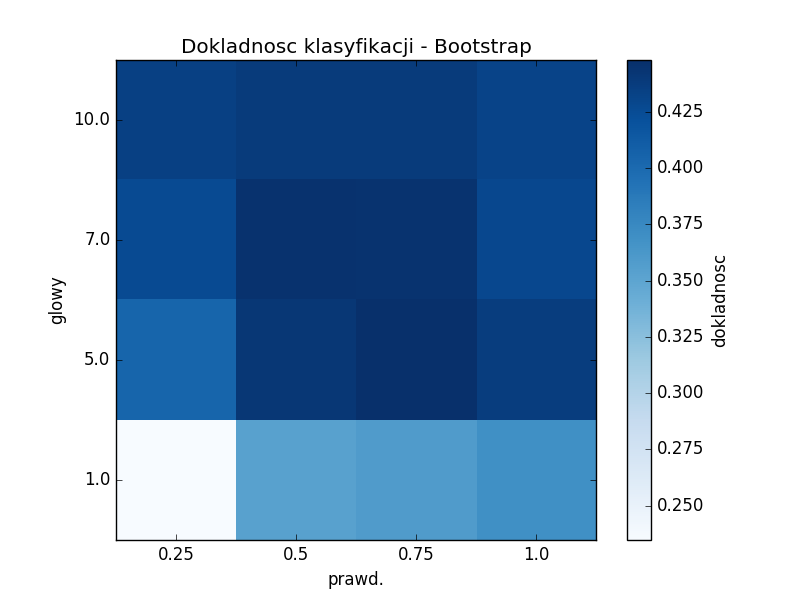
\includegraphics[scale = 0.35]{figures/figures/uncertainties/bootstrap_accuracy_mean.png}}{\caption{Bootstrap}\label{fig:b_acc_mean}}
		\ffigbox{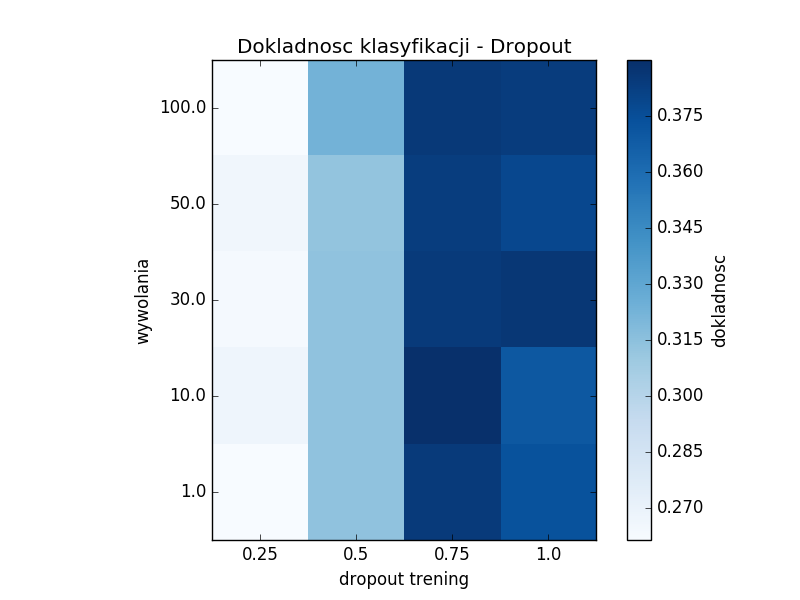
\includegraphics[scale = 0.35]{figures/figures/uncertainties/dropout_accuracy_mean.png}}{\caption{Dropout}\label{fig:d_acc_mean}}
	\end{floatrow}
\end{figure}

\begin{figure}[H]
	\begin{floatrow}
		\ffigbox{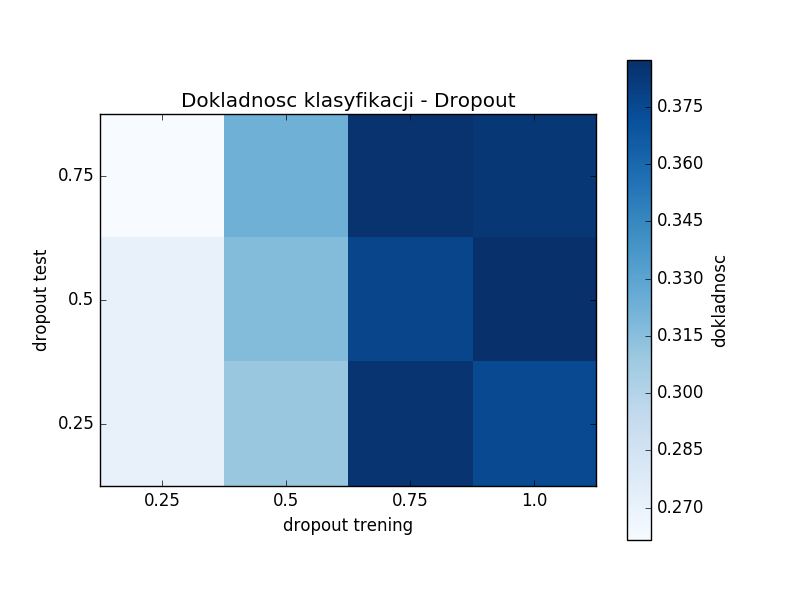
\includegraphics[scale = 0.35]{figures/figures/uncertainties/dropout_accuracy_mean2.png}}{\caption{Dropout}\label{fig:d_acc_mean2}}
		\ffigbox{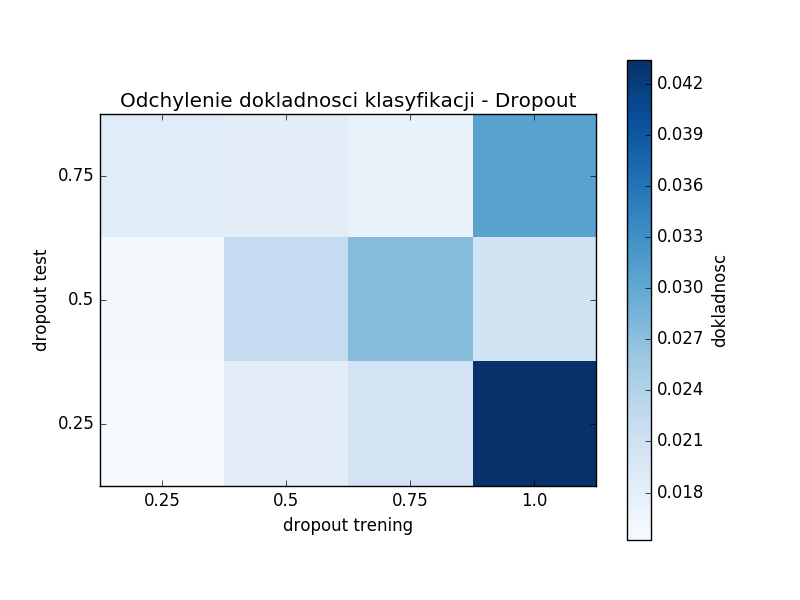
\includegraphics[scale = 0.35]{figures/figures/uncertainties/dropout_accuracy_variance2.png}}{\caption{Dropout}\label{fig:d_acc_var2}}
	\end{floatrow}
\end{figure}

\begin{figure}[H]
	\begin{floatrow}
		\ffigbox{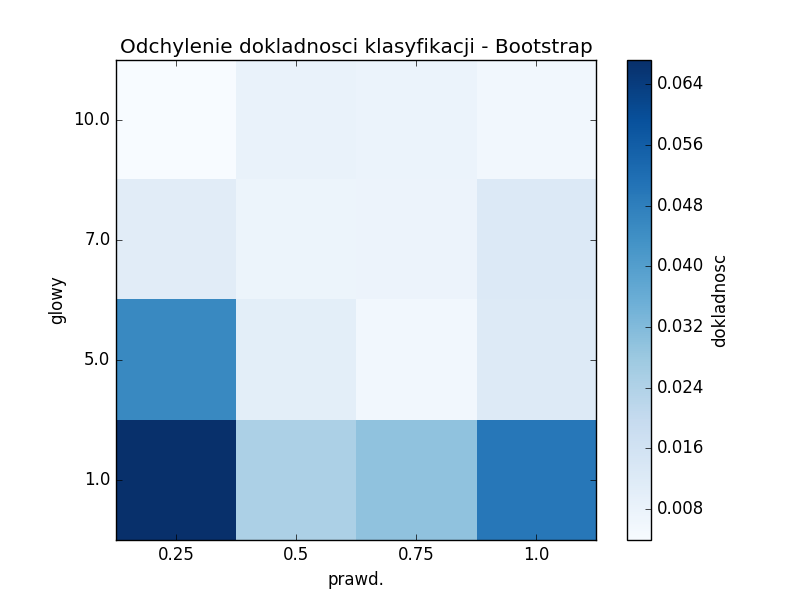
\includegraphics[scale = 0.35]{figures/figures/uncertainties/bootstrap_accuracy_variance.png}}{\caption{Bootstrap}\label{fig:b_acc_var}}
		\ffigbox{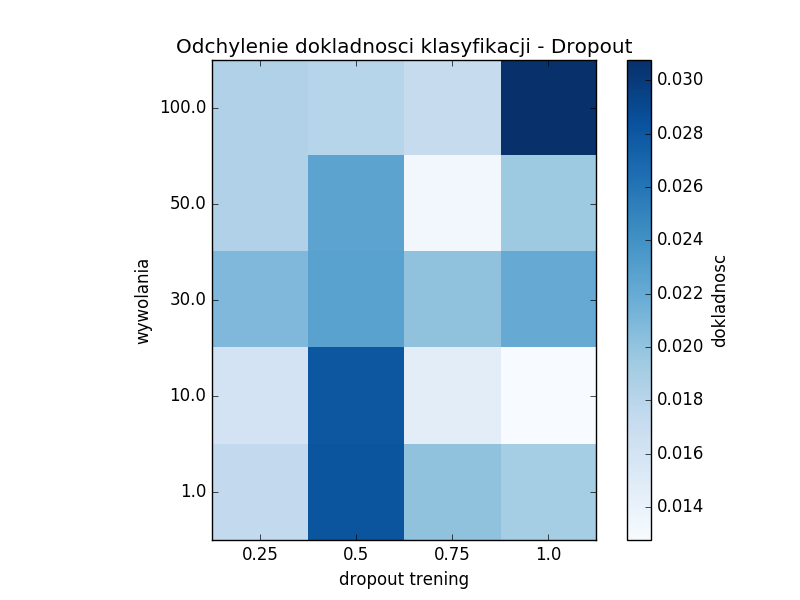
\includegraphics[scale = 0.35]{figures/figures/uncertainties/dropout_accuracy_variance.png}}{\caption{Dropout}\label{fig:d_acc_var}}
	\end{floatrow}
\end{figure}

Na wykresach \ref{fig:b_train_t}, \ref{fig:d_train_t}, \ref{fig:b_test_t}, \ref{fig:d_test_t} przedstawiono czasy treningu i testowania. Na etapie czasu testowania Boostrap wypada znacznie gorzej niż Dropout. 25 sekund dla 5 głów i prawd=0.75 trwa dwa razy dłużej niż 12 sekund osiąganych przez Dropout na wszystkich parametrach, co jest znacznie większym narzutem niż 20\% deklarowane przez autorów metody.

Czas testowania ponownie korzystniejszy jest dla Bootstrapa (0.157s), ponad 5 razy mniej niż Dropout (0.84s). Czas testowania jest bardzo istotny w kontekście Q-learningu, gdzie dla każdej klatki konieczna jest ocena jakości każdego z możliwych ruchów.

Czas treningu Bootstrapa jest w przybliżeniu liniowo zależny od liczby głów pomnożonych przez prawdopodobieństwo uwzględnienia krotki: $t_{train}  \sim n * p_{incl}$, natomiast czas testu jest w przybliżeniu stały. Czas treningu Dropoutu jest w przybliżeniu stały, natomiast czas testu jest w przybliżeniu liniowo zależny od liczby wywołań $t_{test}  \sim n$.
 
Powody znacznych różnic czasowych mogą tkwić w szczegółach implementacji obu metod. Warto zwrócić uwagę, że dla niektórych zastosowań koszt związany z dodatkowymi obliczeniami może być nieakceptowalny. Natomiast dla zastosowań, dla których koszt działania agenta (czyli koszt zbierania próbek danych) przewyższa koszt działania GPU dłuższy czas działania Bootstrapa może być nieistotny, albo zniwelowany przy wykorzystaniu mocniejszych lub większych zasobów. 

\begin{figure}[H]
	\begin{floatrow}
		\ffigbox{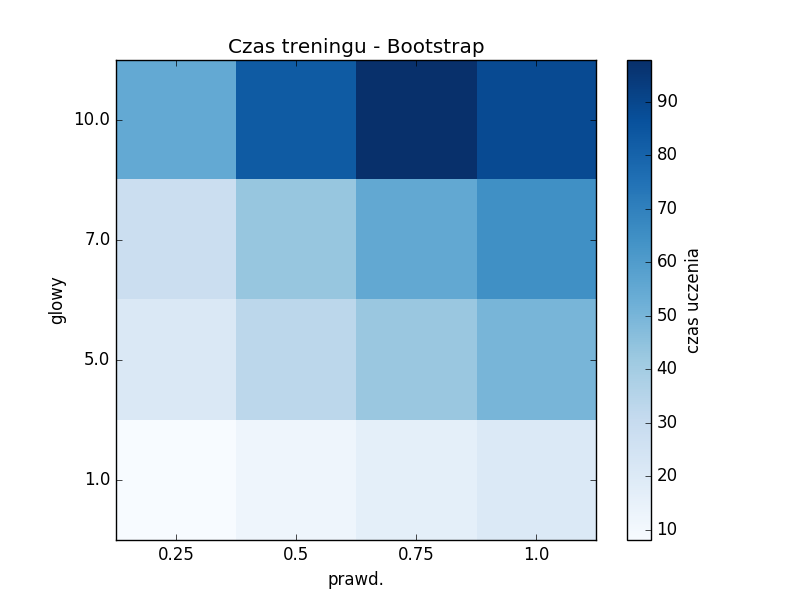
\includegraphics[scale = 0.35]{figures/figures/uncertainties/bootstrap_train_time.png}}{\caption{Dropout}\label{fig:b_train_t}}
		\ffigbox{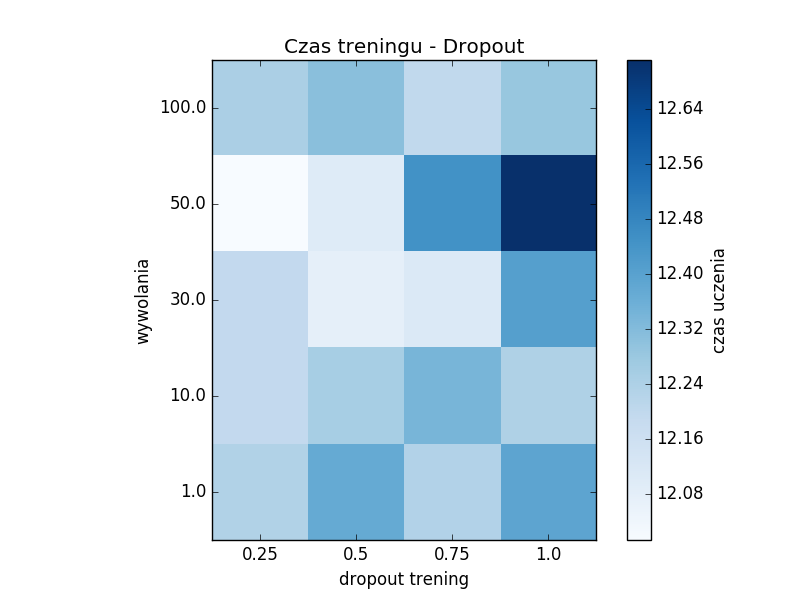
\includegraphics[scale = 0.35]{figures/figures/uncertainties/dropout_train_time.png}}{\caption{Dropout}\label{fig:d_train_t}}
	\end{floatrow}
\end{figure}


\begin{figure}[H]
	\begin{floatrow}
		\ffigbox{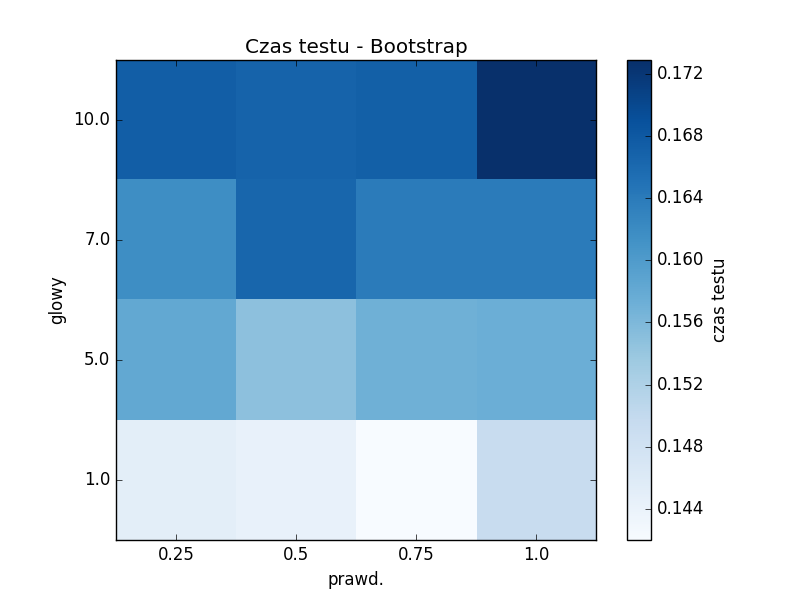
\includegraphics[scale = 0.35]{figures/figures/uncertainties/bootstrap_test_time.png}}{\caption{Dropout}\label{fig:b_test_t}}
		\ffigbox{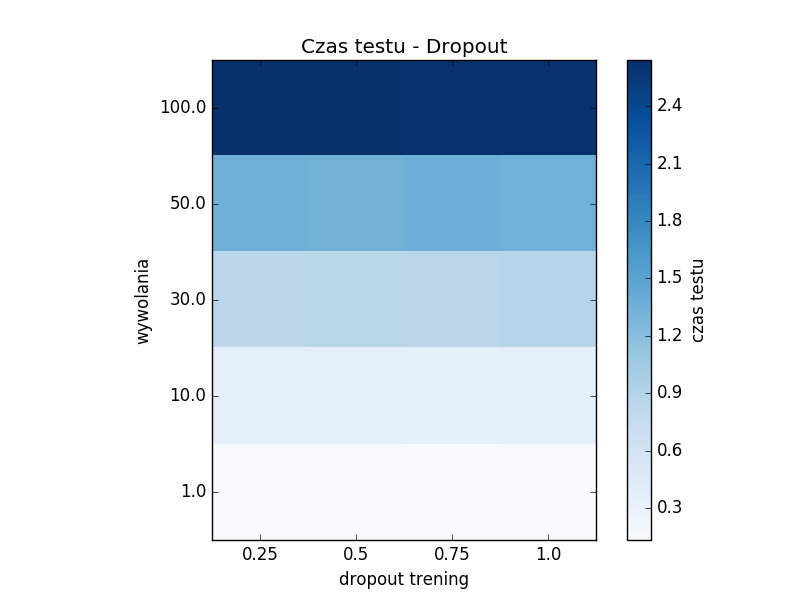
\includegraphics[scale = 0.35]{figures/figures/uncertainties/dropout_test_time.png}}{\caption{Dropout}\label{fig:d_test_t}}
	\end{floatrow}
\end{figure}

Na podstawie przeprowadzonego eksperymentu za najlepszą konfigurację Bootstrapa przyjęto 5 głów i prawdopodobieństwo 0.75, a dla Dropoutu 30 wywołań i oba prawdopodobieństwa równe 0.75

\subsection{Niepewność - wyniki eksperymentu z oceną stopnia pewności}

Dla liczby głów $n=5$ w Bootstrapie i dla liczby wywołań $n=30$ i prawdopodobieństwach dropoutu $p=0.75$ metod współczynnik $quality_{OP}$ dla Bootstrapa z $p=0.75$ wynosi 0.833 przy wariancji 0.11, dla Bootstrapa z $p=1$ wynosi 0.823 przy wariancji 0.10, a dla Dropoutu wynosi 0.925 przy wariancji 0.04. Trafności klasyfikacji dla Bootstrapa z $p=0.75$ wynosi 0.638 a przy wariancji 0.038, dla Bootstrapa z $p=1$ wynosi 0.623 a przy wariancji 0.036 dla Dropoutu wynosi 0.527 przy wariancji 0.032.

\subsection{Niepewność - wnioski}
Bootstrap ma wyraźną przewagę na większości czynników. W drugim eksperymencie jego wyniki są nieznacznie gorsze, ale jako że obie metody osiągają bardzo wysoki współczynnik, ten współczynnik jest pomijalny. Niestety, długi czas treningu Bootstrapa sprawia, że Dropout nie może być kategorycznie odrzucony. Niewykluczone, że w docelowym rozwiązaniu gorsze wyniki Dropoutu będą niezauważalne, natomiast zwiększony czas obliczeń będzie nieakceptowalny.

Najważniejszym wnioskiem jest natomiast obserwacja, że obie metody bardzo skutecznie estymują stopień niepewności.
